% senior_thesis-proposal.tex
% CMPSC 580, Spring 2016
%
%
% This document provides a sample senior thesis proposal template for use
% by students in Allegheny's CS and Applied Computing programs.
%
%   *******************************************************************
%   * LOOK FOR BLOCK COMMENTS SUCH AS THIS ONE FOR AN EXPLANATION OF  *
%   * THIS DOCUMENT AND HOW TO MODIFY IT FOR YOUR OWN PROPOSAL!       *
%   *                                                                 *
%   * ANY LINE BEGINNING WITH A "%" IS A LATEX COMMENT AND IS IGNORED *
%   * BY THE LATEX PROCESSOR. YOU ARE ENCOURAGED TO COMMENT YOUR OWN  *
%   * LATEX CODE.                                                     *
%   *******************************************************************

%   ********************************************************************
%   * THE FIRST SECTION OF THE LATEX FILE IS THE "PREAMBLE." IT        *
%   * INSTRUCTS LATEX TO IMPORT SPECIAL PACKAGES FOR THINGS LIKE       *
%   * INCLUDING FIGURES, DOUBLE-SPACING, COLORED TEXT, ETC.            *
%   * DEPENDING ON YOUR NEEDS, YOU MAY FIND IT NECESSARY TO USE PACK-  *
%   * AGES THAT ARE NOT INCLUDED IN THIS TEMPLATE. SIMPLY IMITATE THE  *
%   * "\usepackage{...}" COMMANDS SHOWN BELOW.                         *
%   ********************************************************************

%   ********************************************************************
%   * BEGINNING OF PREAMBLE:                                           *
%   ********************************************************************
\documentclass[11pt]{article}

\usepackage[T1]{fontenc}
\usepackage{mathptmx}
\topmargin 0.0in
\setlength{\textwidth} {420pt}
\setlength{\textheight} {620pt} 
\setlength{\oddsidemargin} {20pt}
\setlength{\marginparwidth} {72in}

%   ********************************************************************
%   * Many of the commands below were simply copied over from an older *
%   * version of the proposal template; you can just leave them as     *
%   * they are (or you can delve into the TeX/LaTeX documentation      *
%   * and figure out what they do). Otherwise, jump ahead to the next  *
%   * block of comments, where you will enter title, abstract, etc.    *
%   ********************************************************************

\usepackage{fancyhdr} 
\usepackage{url}
\usepackage{graphicx}
\usepackage{cite}

\usepackage{tikz}
\usetikzlibrary{shapes.geometric, arrows}

% set it so that subsubsections have numbers and they
% are displayed in the TOC (maybe hard to read, might want to disable)

\setcounter{secnumdepth}{3}
\setcounter{tocdepth}{3}

% define widow protection

\def\widow#1{\vskip #1\vbadness10000\penalty-200\vskip-#1}

\clubpenalty=10000  % Don't allow orphans
\widowpenalty=10000 % Don't allow widows

% this should give me the ability to use some math symbols that 
% were available by default in standard latex (i.e. \Box)

\usepackage{latexsym}
\usepackage[pdftex,pdfpagelabels,bookmarks,hyperindex,hyperfigures]{hyperref}

% define a little section heading that doesn't go with any number

\def\littlesection#1{
\widow{2cm}
\vskip 0.5cm
\noindent{\bf #1}
\vskip 0.0001cm 
}

\pagestyle{fancyplain}

\newcommand{\tstamp}{\today}   
\renewcommand{\sectionmark}[1]{\markright{#1}}
\lhead[\Section \thesection]            {\fancyplain{}{\rightmark}}
\chead[\fancyplain{}{}]                 {\fancyplain{}{}}
\rhead[\fancyplain{}{\rightmark}]       {\fancyplain{}{\thepage}}
\cfoot[\fancyplain{\thepage}{}]         {\fancyplain{\thepage}{}}

\newlength{\myVSpace}% the height of the box
\setlength{\myVSpace}{1ex}% the default, 
\newcommand\xstrut{\raisebox{-.5\myVSpace}% symmetric behaviour, 
  {\rule{0pt}{\myVSpace}}%
}

% leave things with no spacing extra spacing in the final version of the paper
\renewcommand{\baselinestretch}{1.0}    % must go before the begin of doc
\providecommand{\keywords}[1]{\textbf{\textit{Keywords---}} #1}
% suppress the use of indentation for a paragraph

\setlength{\parindent}{0.0in}
\setlength{\parskip}{0.1in}

\begin{document}


% handle widows appropriately
\def\widow#1{\vskip #1\vbadness10000\penalty-200\vskip-#1}

% build the title section

\makeatletter

\def\maketitle{%
  %\null
  \thispagestyle{empty}%
  %\vfill
  \begin{center}%\leavevmode
    %\normalfont
    {\Huge \@title\par}%
    %\hrulefill\par
    {\normalsize \@author\par}%
    \vskip .4in
%    {\Large \@date\par}%
  \end{center}%
  %\vfill
  %\null
  %\cleardoublepage

  }

\makeatother

%   ********************************************************************
%   * Here is the first place where you need to begin customizing:     *
%   * Enter you name, the title of your proposal, etc., in the places  *
%   * indicated by the comment "% CHANGE!".                            *
%   ********************************************************************

\vspace*{-1.1in}
\title{Measuring the Digital Footprint \\ \Large A Tool for Understanding the Data Collected from Internet Users}  % CHANGE!

% build the author section
\author{
        Zachary M. Shaffer\\  % CHANGE!
        Department of Computer Science\\
        Allegheny College \\
        {\tt shafferz@allegheny.edu}  \\  % CHANGE!
        \url{http://shafferz.github.io} \\  % CHANGE OR DELETE!
        \vspace*{.1in} \today \\ \vspace*{.1in}
}

\maketitle       % use the default title stuff

% Default "abstract" environment is too small; customize one instead:
\begin{center}
\large\bf Abstract
\vspace{-1em}  % Reduce space between header and the abstract
\end{center}

%   ********************************************************************
%   * Here is the second place where you need to customize:            *
%   * enter your abstract in the "quote" environment:                 *
%   ********************************************************************

\begin{quote}
Every week, hundreds of millions of Americans access the internet for billions of hours. In this time, the user generates a distinct digital footprint that can be used to identify the user's personal information and browsing habits, such as legal names, addresses, phone numbers, entertainment viewing habits, social media accounts, email addresses, and much more. These deeply personal dossiers of information can be linked to a given user with a plurality of tools, cookies, and other unique pieces of identifying information. Since most Americans have concerns about their digital privacy, this thesis proposes a tool that will identify, measure, and present a user with their own digital footprint, and give the user advice on how to reduce the transparency of this information. To accomplish this, it will utilize aspects of data collection, machine vision, machine learning, best fit algorithms, and data visualization to educate internet users about safe browsing habits. This tool is being developed on the forefront of an age when digital privacy is a major concern throughout the United States as a topical and poignant subject.
\end{quote}
\keywords{digital footprint, browsing habits, cookies, privacy, data collection, machine vision, machine learning, algorithms, data visualization}
%\vspace*{-.4in}
\section{Introduction}
\label{sec:introduction}
\vspace*{-.1in}

%   ********************************************************************
%   * Enter the text of your introductory section here.                *
%   ********************************************************************

In 2016, the average American internet user spent about 23.6 hours online each week\cite{digital-future}. As of June 30, 2017, there are over 286 million American internet users. That is a collective 6.7 billion hours spent online in America alone, and America only accounts for 9.8\% of all internet usage worldwide\cite{internet-world-stats}. Keeping track of what any one given individual does online, then, should seem to be fairly difficult. That is not the case, however, as websites are using information given by users who access the internet to build and sell profiles of any given individual user. 

This collection of information on a user, known as the user's digital footprint, can tell a website anything ranging from their location and IPv6 address, to what kinds of videos the user likes to watch online, or even what kind of products they like to purchase. The average user, however, is typically unaware of the kind of information they are providing to these websites. The motivation for the creation of a digital footprint measuring tool comes from the simple fact that millions of users who spend billions of hours online do not typically understand what is revealed when interacting with the internet. Furthermore, the issue of privacy online is important to most Americans, as 93\% of American adults want to control who can access their information, and 90\% of American adults want to control what information can be accessed about them\cite{pew-internet}.

The personal information of any given individual user that is recorded digitally is what we will define as a {\bf digital footprint}. In some articles, this is also referred to as a {\it cyber shadow}, {\it electronic footprint}, or {\it digital shadow}, but I will synonymize these terms with digital footprint. This thesis will {\bf not} focus on tracking the digital footprint of corporations, companies, or groups, as multiple commercial tools already exist to help a company measure their "digital footprint," which is often used as a marketing term to describe the length of their commercial outreach, rather than a term associated with user privacy or data security. Furthermore, these tools are largely unhelpful to an individual user for tracking, measuring, or understanding their personal digital footprint. 

\vspace*{-.1in}
\section{Related Work}
\label{sec:relatedwork}
\vspace*{-.1in}

%   ********************************************************************
%   * Enter the text of your related work section here.                *
%   ********************************************************************

\subsection{Free Self-Searching or Person-Searching Tools} \label{sec:free}
Numerous resources exist for directing a user to websites that aid in the process of investigating and measuring your public digital footprint manually. The Centre for the Protection of National Infrastructure in the United Kingdom, for example, produced a simple guide for the common user for discovering and managing their digital footprint\cite{cpni-df}. In the guide, they reference multiple websites that are free to use for discovering the scope of the user's digital footprint, such as \href{http://www.pipl.com}{\it Pipl} for personal information, \href{http://www.whois.com}{\it Whois.com} for information on website owners, and \href{http://www.tineye.com}{\it TinEye} for image searching. Pipl is a search engine that uses deep-diving algorithms to find information that is publicly available and associated with specific names. The searches on Pipl can be refined with email addresses, phone numbers, or locations. Whois.com is a website for searching domains and finding information regarding the websites' owners. TinEye is a reverse-image search engine that takes a digital photo as input and searches the web for it using computer vision, pattern recognition, neural networks, and machine learning \cite{tineye}. None of the aforementioned resources, however, automatically track data of an individual user of the internet. They are strictly manual searches, requiring names or images to be searched manually.

\subsection{Common Techniques for Identifying and Tracking Users} \label{sec:common}
A user's internet browser plays a large role in indentifying any given individual user from the millions of other internet users, which consequently can influence the amount of information associated with a user's digital footprint. The technique of analyzing a user's internet browser to identify them is known as {\bf browser fingerprinting}, and can play a substantial role in identifying a user. {\it \href{https://panopticlick.eff.org/}{Panopticlick}}, a research project by the Electrionic Frontier Foundation, is one tool available for free online to help a user determine the uniqueness of their browser fingerprint\cite{panopticlick}. This technology can help the tool proposed in this thesis further generate an in-depth and personal dossier of a user's browsing habits. The ability to accurately fingerprint and identify a user's browser is, in and of itself, a powerful tool for invading a user's privacy.

To discuss or investigate measuring a user's digital footprint without discussing {\bf trackware} or {\bf tracking cookies} would be like discussing identifying cars without mentioning license plates. Trackware is, in broad terms, any piece of software that tracks system or user activity. Tracking cookies are a type of trackware deployed by websites to uniquely identify a visitor. One open-source tracking cookie is \href{https://samy.pl/evercookie/}{\it evercookie}, an aggressively persistent cookie that restores deleted cookie data everywhere if any piece of the cookie remains on the user's system\cite{evercookie}. Paired with previously mentioned tools, tracking cookies can be created and implemented to further increase the effectiveness of the proposed tool. Furthermore, while addressing tracking cookies, {\bf supercookies} must also be identified as a serious threat to user privacy online. The definitions of a supercookie vary depending on source, ranging from a specific packet of information injected by Internet Service Providers (ISPs) like Comcast or Verizon containing unique HTTP headers that store personal information \cite{supercookie-definition}, to any cookie that is designed to be stored permanently on a user's computer. For the purpose of this thesis, the latter definition will be used, as it is more accurate to the usage of the term in research conducted thus far associated with this thesis.

\vspace*{-.2in}
\section{Method of Approach}
\label{sec:method}
\vspace*{-.1in}

%   ********************************************************************
%   * Enter the text of your method of approach section here.          *
%   ********************************************************************

\tikzset{every picture/.style={line width=0.75pt}} %set default line width to 0.75pt        
\begin{tikzpicture}[x=0.75pt,y=0.75pt,yscale=-1,xscale=1]
%uncomment if require: \path (0,425); %set diagram left start at 0, and has height of 425
\draw    (252, 6) rectangle (342, 46)   ;
\draw [rotate around= { 46.19: (295.51, 117.86)
    }]   (244.68, 67.04) rectangle (346.33, 168.69)   ;
\draw    (6, 89) rectangle (184, 166)   ;
\draw    (455, 120) rectangle (607, 180)   ;
\draw    (438, 1) rectangle (623, 79)   ;
\draw    (444, 215) rectangle (621, 257)   ;
\draw    (416, 284) rectangle (651, 326)   ;
\draw    (368,150) -- (455,150) ;
\draw [shift={(455,150)}, rotate = 180] [color={rgb, 255:red, 0; green, 0; blue, 0 }  ]   (0,0) .. controls (3.31,-0.3) and (6.95,-1.4) .. (10.93,-3.29)(0,0) .. controls (3.31,0.3) and (6.95,1.4) .. (10.93,3.29)   ;
\draw    (59,304) -- (366,302) ;
\draw    (223.65,116.37) -- (185.65,116.37) ;
\draw [shift={(185.65,116.37)}, rotate = 360] [color={rgb, 255:red, 0; green, 0; blue, 0 }  ]   (0,0) .. controls (3.31,-0.3) and (6.95,-1.4) .. (10.93,-3.29)(0,0) .. controls (3.31,0.3) and (6.95,1.4) .. (10.93,3.29)   ;
\draw    (367.37,119.35) -- (413,119) ;
\draw    (413,119) -- (413,42) ;
\draw    (413,42) -- (438,40) ;
\draw [shift={(438,40)}, rotate = 535.4300000000001] [color={rgb, 255:red, 0; green, 0; blue, 0 }  ]   (0,0) .. controls (3.31,-0.3) and (6.95,-1.4) .. (10.93,-3.29)(0,0) .. controls (3.31,0.3) and (6.95,1.4) .. (10.93,3.29)   ;
\draw    (530.5,79) -- (531,120) ;
\draw [shift={(531,120)}, rotate = 269.3] [color={rgb, 255:red, 0; green, 0; blue, 0 }  ]   (0,0) .. controls (3.31,-0.3) and (6.95,-1.4) .. (10.93,-3.29)(0,0) .. controls (3.31,0.3) and (6.95,1.4) .. (10.93,3.29)   ;
\draw    (531,180) -- (532.5,215) ;
\draw [shift={(532.5,215)}, rotate = 267.55] [color={rgb, 255:red, 0; green, 0; blue, 0 }  ]   (0,0) .. controls (3.31,-0.3) and (6.95,-1.4) .. (10.93,-3.29)(0,0) .. controls (3.31,0.3) and (6.95,1.4) .. (10.93,3.29)   ;
\draw    (532.5,257) -- (533.5,284) ;
\draw [shift={(533.5,284)}, rotate = 267.88] [color={rgb, 255:red, 0; green, 0; blue, 0 }  ]   (0,0) .. controls (3.31,-0.3) and (6.95,-1.4) .. (10.93,-3.29)(0,0) .. controls (3.31,0.3) and (6.95,1.4) .. (10.93,3.29)   ;
\draw    (653,40) -- (651,284) ;
\draw    (653,40) -- (623,40) ;
\draw [shift={(623,40)}, rotate = 360] [color={rgb, 255:red, 0; green, 0; blue, 0 }  ]   (0,0) .. controls (3.31,-0.3) and (6.95,-1.4) .. (10.93,-3.29)(0,0) .. controls (3.31,0.3) and (6.95,1.4) .. (10.93,3.29)   ;
\draw    (95,223) -- (95,166) ;
\draw    (295,222) -- (95,223) ;
\draw    (295,222) -- (294.01,189.72) ;
\draw [shift={(294.01,189.72)}, rotate = 448.25] [color={rgb, 255:red, 0; green, 0; blue, 0 }  ]   (0,0) .. controls (3.31,-0.3) and (6.95,-1.4) .. (10.93,-3.29)(0,0) .. controls (3.31,0.3) and (6.95,1.4) .. (10.93,3.29)   ;
\draw    (59,165) -- (59,304) ;
\draw    (366,302) -- (368,150) ;
\draw    (386,236) -- (444,236) ;
\draw    (386,236) -- (386,326) ;
\draw    (297,326) -- (386,326) ;
\draw    (297,326) -- (297,361) ;
\draw [shift={(297,361)}, rotate = 270] [color={rgb, 255:red, 0; green, 0; blue, 0 }  ]   (0,0) .. controls (3.31,-0.3) and (6.95,-1.4) .. (10.93,-3.29)(0,0) .. controls (3.31,0.3) and (6.95,1.4) .. (10.93,3.29)   ;
\draw    (25, 362) rectangle (359, 424)   ;
\draw    (359,393) -- (420,393.5) ;
\draw [shift={(420,393.5)}, rotate = 180.47] [color={rgb, 255:red, 0; green, 0; blue, 0 }  ]   (0,0) .. controls (3.31,-0.3) and (6.95,-1.4) .. (10.93,-3.29)(0,0) .. controls (3.31,0.3) and (6.95,1.4) .. (10.93,3.29)   ;
\draw    (420, 363) rectangle (623, 424)   ;
\draw (298,26) node  [align=left] {Install Tool};
\draw (296,118) node  [align=left] { \ \ \ Do we know\\the email address\\ \ \ \ \ of the user?};
\draw (95,128) node  [align=left] {Use tracking cookies and\\ browser fingerprinting to\\ \ \ attempt to identify the \\ \ \ user's email address.};
\draw (531,40) node  [align=left] {Use Pipl API to search for\\ usernames, legal names,\\and addresses associated\\ \ \ \ \ with data collected.};
\draw (534,305) node  [align=left] {Fetch collected data from tracking\\ \ cookies and browser fingerprint.};
\draw (532,236) node  [align=left] { Visualize and verify the\\information with the user.};
\draw (531,150) node  [align=left] {Generate an XML file\\ \ with any/all known\\ data about the user.};
\draw (209,293) node  [align=left] {After 30 Days};
\draw (190,212) node  [align=left] {Within 30 Days};
\draw (388,109) node  [align=left] {Yes};
\draw (211,106) node  [align=left] {No};
\draw (192,393) node  [align=left] { Prepare and produce an "exit plan" for the user,\\ advising them on how to proceed with improving\\ \ \ \ \ \ \ \ \ \ \ \ \ \ \ \ their web browsing security.};
\draw (342,316) node  [align=left] {User Quits};
\draw (522,393) node  [align=left] {Terminate any acquired data,\\planted cookies, or local files\\ remaining on user's system.};
\end{tikzpicture}
\begin{center}
\label{fig:fig1} Figure 1. An Overview of the Proposed Tool's Mechanics.
\end{center}

\subsection{Identifying and Tracking Specific Users} \label{sec:identifying}
The first step of the proposed thesis is to identify free and open-source software that can be used to identify an individual user, and for this the information found when researching for section \ref{sec:common} will be useful. The first step towards this goal will be to utilize a tracking cookie that can be deployed from a simple webpage. For this, the tool will use the evercookie \cite{evercookie}. Evercookie uses a list of vulnerabilities and methods for storing data on the user's browser, and, if up to all but one the storage mechanisms fail or are wiped clean, the cookie has the ability to regenerate itself entirely using any remaining fragments of it's data. The storage mechanisms that the evercookie utilizes specifically are: 
\begin{itemize}
  \item Standard HTTP Cookies.
  \item HTTP Strict Transport Security (HSTS) Pinning.
  \item Local Shared Objects (Flash Cookies).
  \item Silverlight Isolated Storage. 
  \item Storing cookies in RGB values of auto-generated, force-cached PNGs using HTML5 Canvas tag to read pixels (cookies) back out.
  \item Storing cookies in Web History. 
  \item Storing cookies in HTTP ETags. 
  \item Storing cookies in Web cache. 
  \item window.name caching.
  \item Internet Explorer userData storage.
  \item HTML5 Session Storage. 
  \item HTML5 Local Storage.
  \item HTML5 Global Storage.
  \item HTML5 Database Storage via SQLite.
  \item HTML5 IndexedDB.
  \item Java JNLP PersistenceService.
  \item Java applet sandbox escaping exploitation.
\end{itemize}
Evercookie, paired with a service similar to Panopticlick\cite{panopticlick}, can go a long way towards identifying the unique user. Peter Eckersley, \href{https://panopticlick.eff.org/static/browser-uniqueness.pdf}{in his report on the Panopticlick tool}, discuss how relatively simple it is to perform a task like browser fingerprinting, and warns that these fingerprinted records are potentially personally identifiable \cite{panopticlick-report}. Furthermore, in their methodology, they describe the process of browser fingerprinting, and the possible extent to which fingerprinting can identify a user. By simple string concatenation, the Panopticlick tool creates a long string representation of the user's browser fingerprint by collecting the data readily and publicly accessed by a website via simple, static HTTP requests, as well as common AJAX (Asynchronous JavaScript and XML) techniques. For this thesis, though, a similar open sourced tool may be substituted in place of Panopticlick, or some other from-scratch implementation.

As Eckersley warns, there are multiple stages to potentially tracking a user. The first stage, or "test" of a user who does not wish to be tracked as they use the web, is to find appropriate settings for blocking and restricting tracking cookies without limiting web usability or interface interaction. The proposed tool will amplify the difficulty of this stage, as the use of the aforementioned evercookie, or similar supercookies, will make finding comfortable settings for the user more difficult, if not impossible or irrelevant. The volume of users who make it through this obstacle will be drastically reduced immediately. The second stage that Eckersley defines for the user would then be for the user to research various supercookies and ways to disable them. Provided appropriate implementation, this stage will also be extremely difficult for the user to complete. With the number of users who can successfully cirvumvent or avoid measures taken by the tool to utilize tracking cookies and supercookies reduced to a notable minority, the remaining users would then need to overcome the tool's use of browser fingerprinting. This is nearly impossible, as Eckersley points out, as browser fingerprinting ``has the insidious property that it\dots leaves no persistent evidence of tagging on the user's computer.'' \cite{panopticlick-report}

Eckersley goes on to describe the mathematical analysis of the algorithm used by the Panopticlick tool, as well as the methods the tool uses to identify the fingerprint. He also mentions that there are things that went unimplemented in the tool that may exist in commercial software, due to time and knowledge limitations presented in the creation of the tool. One footnote even mentions that some commercial softwares claim to be able detect irregularities in the TCP/IP stack and pierce through proxy servers. Ideally, the proposed tool will be able to do something similar, but this thesis may encounter similar limitations to that which Eckersley faced, and therefore may not have the time to implement such an extention. If further developed beyond the scope of the senior thesis project, this would be a feature greatly desired and worked at independently. With this final possibility, it is clear that commercial tools already exist that can identify a unique user, with or without cookies, amongst other identifiable information. Once this information is acquired, the tool will move on to attempt a more personal analysis.

\subsection{Utilizing Tracking Information to Identify Personal Aspects of Users' Lives} \label{sec:utilizing}
To acquire more personal information, the strategy the tool will employ is to attempt to gather any or all of the following information utilizing the aforementioned tracking methods, and put them through searches based on the tools from section \ref{sec:free}:

\begin{itemize}
\item Preferred and/or legal name.
\item Current or former email address(es).
\item Current or former phone number(s).
\item Current or former location(s) of residency.
\item Current or former usernames.
\item Age.
\end{itemize}

Depending on the success of the acquisition of information, the tool may be able to produce a comprehensive report that gathers and updates the remaining missing information. In the best case scenario for the tool, a simple preliminary scan of already existing information stored in cookies may be able to successfully do this. If this initial information search proves suboptimal or unfruitful, the tool may continue to monitor and track the user's activity over the course of and up to 30 days, or until it has acquired any of the above information. This can be done by reading the headers of a website, but may be difficult to do. Another option is to try to capture packets of information containing other websites' cookies and decrypt/dehash them, but there are two issues with this. First, cookies are time-sensitive so this may not be feasible. Second, this is not legal and therefore not a valid solution. If any of the information is successfully acquired by the tool, though, it will use an open-source API of the Pipl engine to search usernames, legal names, phone numbers, or other information associated with the email address\cite{pipl-api}. After using the Pipl search engine on my own email addresses, I was able to yield my full legal/preferred name, current home address, previous home addresses, former telephone numbers, and links to my social media accounts, which yields 5/6 of the aforementioned pieces of information with a simple one-time search. Furthermore, it also presented me with the names and information of my relatives, an aspect of the tool that was never intended to be tracked before this revelation. This Pipl API is open source, free, and supported across multiple programming languages. The simple Java library implementation will suffice for the purposes of this tool.

Finally, an optimistic goal of this thesis is to implement a method of acquiring a photo of the user. Upon consideration, there are two ways that this can be done, one of which may be considered overtly invasive, concerning, or may even require special agreement by the user in advance.
\begin{enumerate}
\item The first option is to allow the tool to attempt to use the user's webcam in a clandestine manner to capture a screenshot of their face. From here, their face can be put through a simple Google image search along with their name, and potentially yield photos of the user based on their name and what they look like. This may require the user to digitally sign an agreement waiving liability of the tool, or some other legal protocol, as I cannot imagine this process being otherwise legal. This option, however, would be the most effective in conveying the extent to which websites can go to identify a user.

\item The second option would be to simply allow the user to upload their own self portrait, and perform the same search as described above. The notion of secretly accessing the user's webcam can be described to the user, and a similar result can be yielded, but this method provides significantly less of a shock'' effect. This option does seem to be the more likely of the two, though, for obvious ethical and legal reasons.
\end{enumerate} 

Once the aforementioned data is collected, and the tool has run for a sufficient amount of time, a simple text-processing application or module can be implemented in Java to organize and structure the output of the data, organize the filesystem of the collected data, and yield a structured {\tt output.xml} file. An XML file can be useful to help organize collected data in a way that is easy for both machines and humans to read, which will be invaluable in the early developmental stages. The XML file can then be read by another program or piece of code to produce a graphical output for the user in the end-product.

\subsection{Data Visualization} \label{sec:data}
Once the information has been gathered by the tool, the ultimate goal of the project can be realized through data sorting and presentation, in the form of an interactive graphical user interface presented to the user. If acquired, the tool will show the user a picture of themselves (preferrably one that the user did not automatically give to the tool) and their name in large, legible print across the top of what would look similar to a social media biography page. This part of the tool can be built using a combination of Java and HTML, to produce either a simple graphical layout via backend software, or even by producing an HTML web-page based on a pre-configured HTML5/CSS template.

While this output may appear to be similar to the front page of a personal website, resume, or social media application, the context provided by the manner in which the information was collected will, ideally, have a chilling or discomforting effect. The user, depending on the accuracy of the reported information, may feel shocked by or afraid of the information that they did not know they may have been willingly releasing to the online public. Users whose reports come back largely incorrect or sparse, however, may feel significantly different. The user may feel relieved by or confident in their safer or more secure browsing habits. While the former reaction is both what is predicted to be the result and preferred, the most likely scenario is a reaction or result somewhere in the middle. Once the data is simplified and organized in this manner, a similar Java or JavaScript applet will be implemented to allow the user to refactor the data if they choose. The purpose of this step is to accomplish two things. First, if the initial presentation of the collected data is inaccurate and the user is feeling confident, the user can potentially be shown that the tool is only one or two simple steps away from creating a more accuracante profile. Second, this gives the program potentially useful data for future usage or improvement, opening the opportunity to implement machine learning into the tool and further automate and improve the accuracy of the process of data collection.

\subsection{End of Software Life and Closing Note} \label{sec:end}
The process of user-guided data refactorization can be repeated, and it will be the responsibility of the user to verify the accuracy of the tool at this stage. Whenever the user decides they have used the tool for long enough, or are satisfied with the end result of the tool, it will then try to help the user identify ways to improve their own personal security. First, it will recommend steps and existing software that exists to attempt to counter unwanted digital surveilance. This includes regularly vetting their own browser cookies, using virtual proxy networks (VPNs) to mask internet usage and confuse tracking software, and using browsers that are pre-configured for maximum personal security. The tool will eventually also support built-in methods of automated cookie and cache cleaning that both helps improve the user's privacy and incentivizes the user to continue to use the tool. If the user decides that they do not wish to use the tool any longer and is ready to uninstall it, the tool will automatically perform this function as part of the uninstallation process. This is to maximize personal user privacy, and works to erase any and all data accrued by the tool that the user may feel is sensitive or private. 

Notice that at no point in this methodology is transmitting the user's data to a database for long-term storage or access by the creator ever mentioned or proposed. This is because I feel that if a tool of this nature were to do such a thing, it would be the most egregious form of malicious hypocrisy. This tool is not and will never be, for as long as it is in my control, a commercially available software, nor will it ever have the capability to be converted into such. For similar reasons, the end-product, if successful, must be designed with careful attention to the security details in the code, and will not be released open-source, despite being built largely on the shoulders of open-sourced software. If this is not legally possible, the final product may be intentionally faulty or incomplete, in the interest of preserving the privacy of all internet users.

\vspace*{-.2in}
\section{Evaluation Strategy}
\label{sec:evaluate}
\vspace*{-.1in}

%   ********************************************************************
%   * Enter the text of your evaluation strategy section here.         *
%   ********************************************************************

\subsection{User-Guided Evaluation} \label{sec:user}
The tool will be largely evaluated by the user of the software, and will ideally use feedback from users to improve the accuracy and usefulness of results of the scale up to and through final deployment. User curation and feedback will help me to know what kind of information is useful in the future. This will be done by creating a separate piece of software that anonymizes the collected data from the base tool. With the data cloned and anonymized, it will copy the user's feedback applied to the results of the tool as described in sections \ref{data} and \ref{end}. Using the user's feedback choices with anonymized data will be able to generate accuracy data without necessarily conveying the specific details of the data. This evaluation method may seem overly complex, but it is optimal for preserving the user's privacy. If it can be done within the scope of the project, a future goal for the project would be to implement some level of machine learning to the tool for learning how a user will behave online. This can be done with a neural network, linear regression, or some other machine learning technique. The number input can be taken from the previously mentioned user feedback data. 

Beyond the technical results of the tool, the user can also optionally participate in an exit survey. The purpose of the survey will be to evaluate the look and feel of the tool, the aesthetic design of the produced results, and opinions of the user regarding the degree of helpfulness of the tool. The user can also provide input for the usefulness of the advice given at the end of the program, as well as the part of the tool that allows the user to semi-automatically discharge unwanted tracking software from their system. This type of review is typically done for marketing purposes, but the goal of the thesis is to provide genuine improvements to personal safe browsing habits and this style of exit survey may be the best way to understand how to properly communicate complex computer science ideas to the average user for their own benefit.

\subsection{Software Functionality Testing} \label{sec:software}

Testing and evaluation performed during the development stages of the software will be difficult. As indicated in Figure 1, the tool will ideally use a 30-day buffer period to attempt to acquire as much data that it can about the user. If the tool cannot acquire much information, I speculate that it will struggle to acquire any information whatsoever. This is because things like a user's real name and address are inherently difficult to obtain, as that information is typically only either freely given by the user (if we are lucky), or withheld by the user's Internet Service Provider. Tracking cookies and browser fingerprinting can still colelct an impressive amount of data on an individual user, but with limited amounts of information, particularly personal and/or shocking information may be hard to come by. For this reason, a large period of time should be given to the tool to have the opportunity to find this information, with regular refreshes to check whether or not email has been found. This creates an interesting difficulty within testing the software, as trial runs of the program would take literal months to complete on any given machine. To circumvent this, I would attempt to deploy the software for testing to a research or trial group of volunteers. Many previous theses have struggled when it came to the aspect of getting and relying on volunteers, and for a comprehensive project that deals with data as sensitive as this, it may be more difficult. 

Testing the individual components of the software, though, will be relatively simple and straightforward. Since the tool can be written almost exclusively in Java, much of the software will be able to be run against a customized JUnit test suite. This will allow analysis of runtime, efficiency of algorithmic calculations, and the ability to test the basic functions and aspects of the tool. This will be an absolutely necessary step of development, considering that this thesis is largely modular in nature. This means that many aspects of this tool may go wrong, and having a strong automated testing environment will alleviate many stressors and unforeseeable issues by helping to identify specific aspects of the program that fail to function properly. 

\vspace*{-.1in}
\section{Conclusion}
\label{sec:conclusion}
\vspace*{-.1in}

%   ********************************************************************
%   * Enter the text of your concluding section section here.          *
%   ********************************************************************

I believe that the impact of the proposed research has ramifications that supercede the field of Computer Science. In the contemporary digital age, users of the internet worldwide are more connected than ever. We, as a society, largely prioritize building a digital life online for others to see over the practicality of safe browsing habits. Our day to day interactions with the internet drive us together, but can also drive us apart. The average user leaks data from their fingertips onto their internet selves, and it is this precise data hemorrhaging that the average user does that has enabled the rise of web brigades, popularly referred to as Russian ``troll farms,'' designed to use easily accessible online data on users to spread misinformation and propaganda. The collection and sale of a user's data is also in the American public eye with regards to Facebook CEO Mark Zuckerberg's Congressional hearings, with regards to a massive data scrape performed by a third party company that violated the privacy of millions of users. In the coming years, both the private sector and governments will be making huge changes to policies and regulations with regards to personal information privacy. This tool has the potential to both inform and frighten the average user into understanding the importance of carefully curating their online exposure and how much data they reveal about themselves online.

The proposed tool will be on the forefront of this monumental wave of changes to user data usage, privacy, and online profiling of users. It will exist in a time when almost every American is aware of digital security concerns associated with using the internet and social media. It is, and always has been, among my greatest concerns to make sure that people are accutely aware of the exact nature of the internet. The software that I am proposing to create and release has, very likely, already been created. This software could already be in use for companies trying to gain an advantage in selling users products, governments attempting to persuade a large audience in their favor, or, even more likely, hackers and cybercriminals who have malicious intentions towards both targetted untargetted users. The thesis should overall encourage users to really learn about what it means to use the internet, how it specifically works, and what they can do to be safer online.

\bibliographystyle{IEEEtran}
\bibliography{IEEEabrv,senior_thesis_proposal}

\end{document}

